One method of machine learning, although not mainly used for dimensional reduction (there are some researchers that have studied the feature selection using them as \cite{sugumaran2007feature} and \cite{cho2011decision}), that takes into account a given classification is Decision Trees. A Decision Tree \citep{rokach2008data} is a prediction model, which given a set of data, makes logical construction diagrams, very similar to rule-based prediction systems, which serve to represent and categorize a series of conditions that occur successively, for the resolution of a problem. There are many algorithms to implement them, we are going to use an optimised version of the CART algorithm \citep{breiman1984classification} with entropy as its criterion.

The advantages of Decision Trees are that they take into account the defined categorisation, as it is a supervised machine learning classification method, and that they are very explainable. However, our purpose is to know the features that best describe the writing style based on the recipient, instead of classifying new messages. For this reason, we are going to make use of the structure of the constructed Decision Tree in order to measure the importance that each style metric has in it.

A good intuition is to think that, in order to study the importance of a node, it is important to bear its depth in the tree in mind, because as lower is as more elements it differentiate. However, it will not be so useful if it just separate elements of the same class. Likewise, the number of samples that reach the node and its category is an important factor to keep in mind. Nevertheless, it will not be helpful if it maintains the proportion of each category in its child nodes. We are able to think many parameters that can have relevance in the definition of the importance of a node in the Decision Tree. In this case we are going to use the Gini Importance \citep{breiman2001random}, which is defined by the following expression:

$$
ni_j = w_jH_j - w_{left(j)}H_{left(j)} - w_{right(j)}H_{right(j)}
$$

Where $ni_j$ is the importance of node j, $w_j$ is the weighted number of samples reaching node j, $H_j$ is the entropy of node j, $left(j)$ is the child node from left split on node j and $right(j)$ is the child node from right split on node j. Consequently, the importance of each feature is defined by the following formula:

$$
fi_i = \frac{\sum_{j\in Nod(i)}ni_j}{\sum_{j\in Nod}ni_j}
$$

Where $fi_i$ is the importance of feature i, $Nod(i)$ is the set of nodes which split on feature i and $Nod$ is the set of all nodes. In our study we are going to use the normalised feature importance, which is defined by the following expression:

$$
nfi_i=\frac{fi_i}{\sum_{j\in F}fi_j}
$$

\begin{figure}
	\centering%
	\centerline{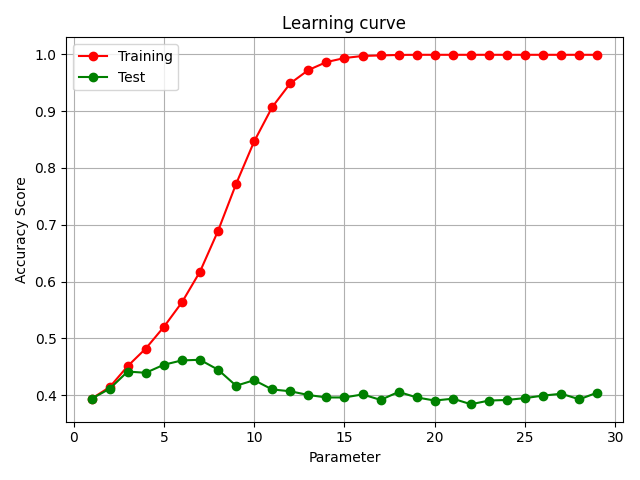
\includegraphics[width=0.7\textwidth]{Imagenes/Bitmap/DecisionTrees/learning28curve.png}}%
	\caption{Learning curve with the 28 chosen features}%
	\label{fig:learn28curve}
\end{figure}

Where $nfi_i$ is the normalised feature importance and $F$ is the set of features. Once we have the expression required for the analysis of the importance of each feature, we are able to calculate the distribution of the importance of each style metric with our 28 chosen style markers. To build the Decision Tree, we have to decide the depth of it. To take this decision, we calculate the learning curve both in training set and test set, and obtain the curves that we can observe in Figure \ref{fig:learn28curve}. Thus, we will choose a depth that avoids the overlearning (which could be produced in values of depth with which the training accuracy score is 1) and the missing of information (depth with which the training accuracy score is less than 0.9). Our choice will be the depth whose training accuracy score is the interval $(0.9, 1)$ and its test accuracy score is maximum (in this case it is eleven, but later, when we had less features, it will follow this criteria).

Making use of the explained expressions for the calculation of the normalised feature importance, we can go through the created tree with the chosen depth in order to obtain the distribution of this value. The result is shown in Figure \ref{fig:nfi28}.

\begin{figure}
	\centering%
	\centerline{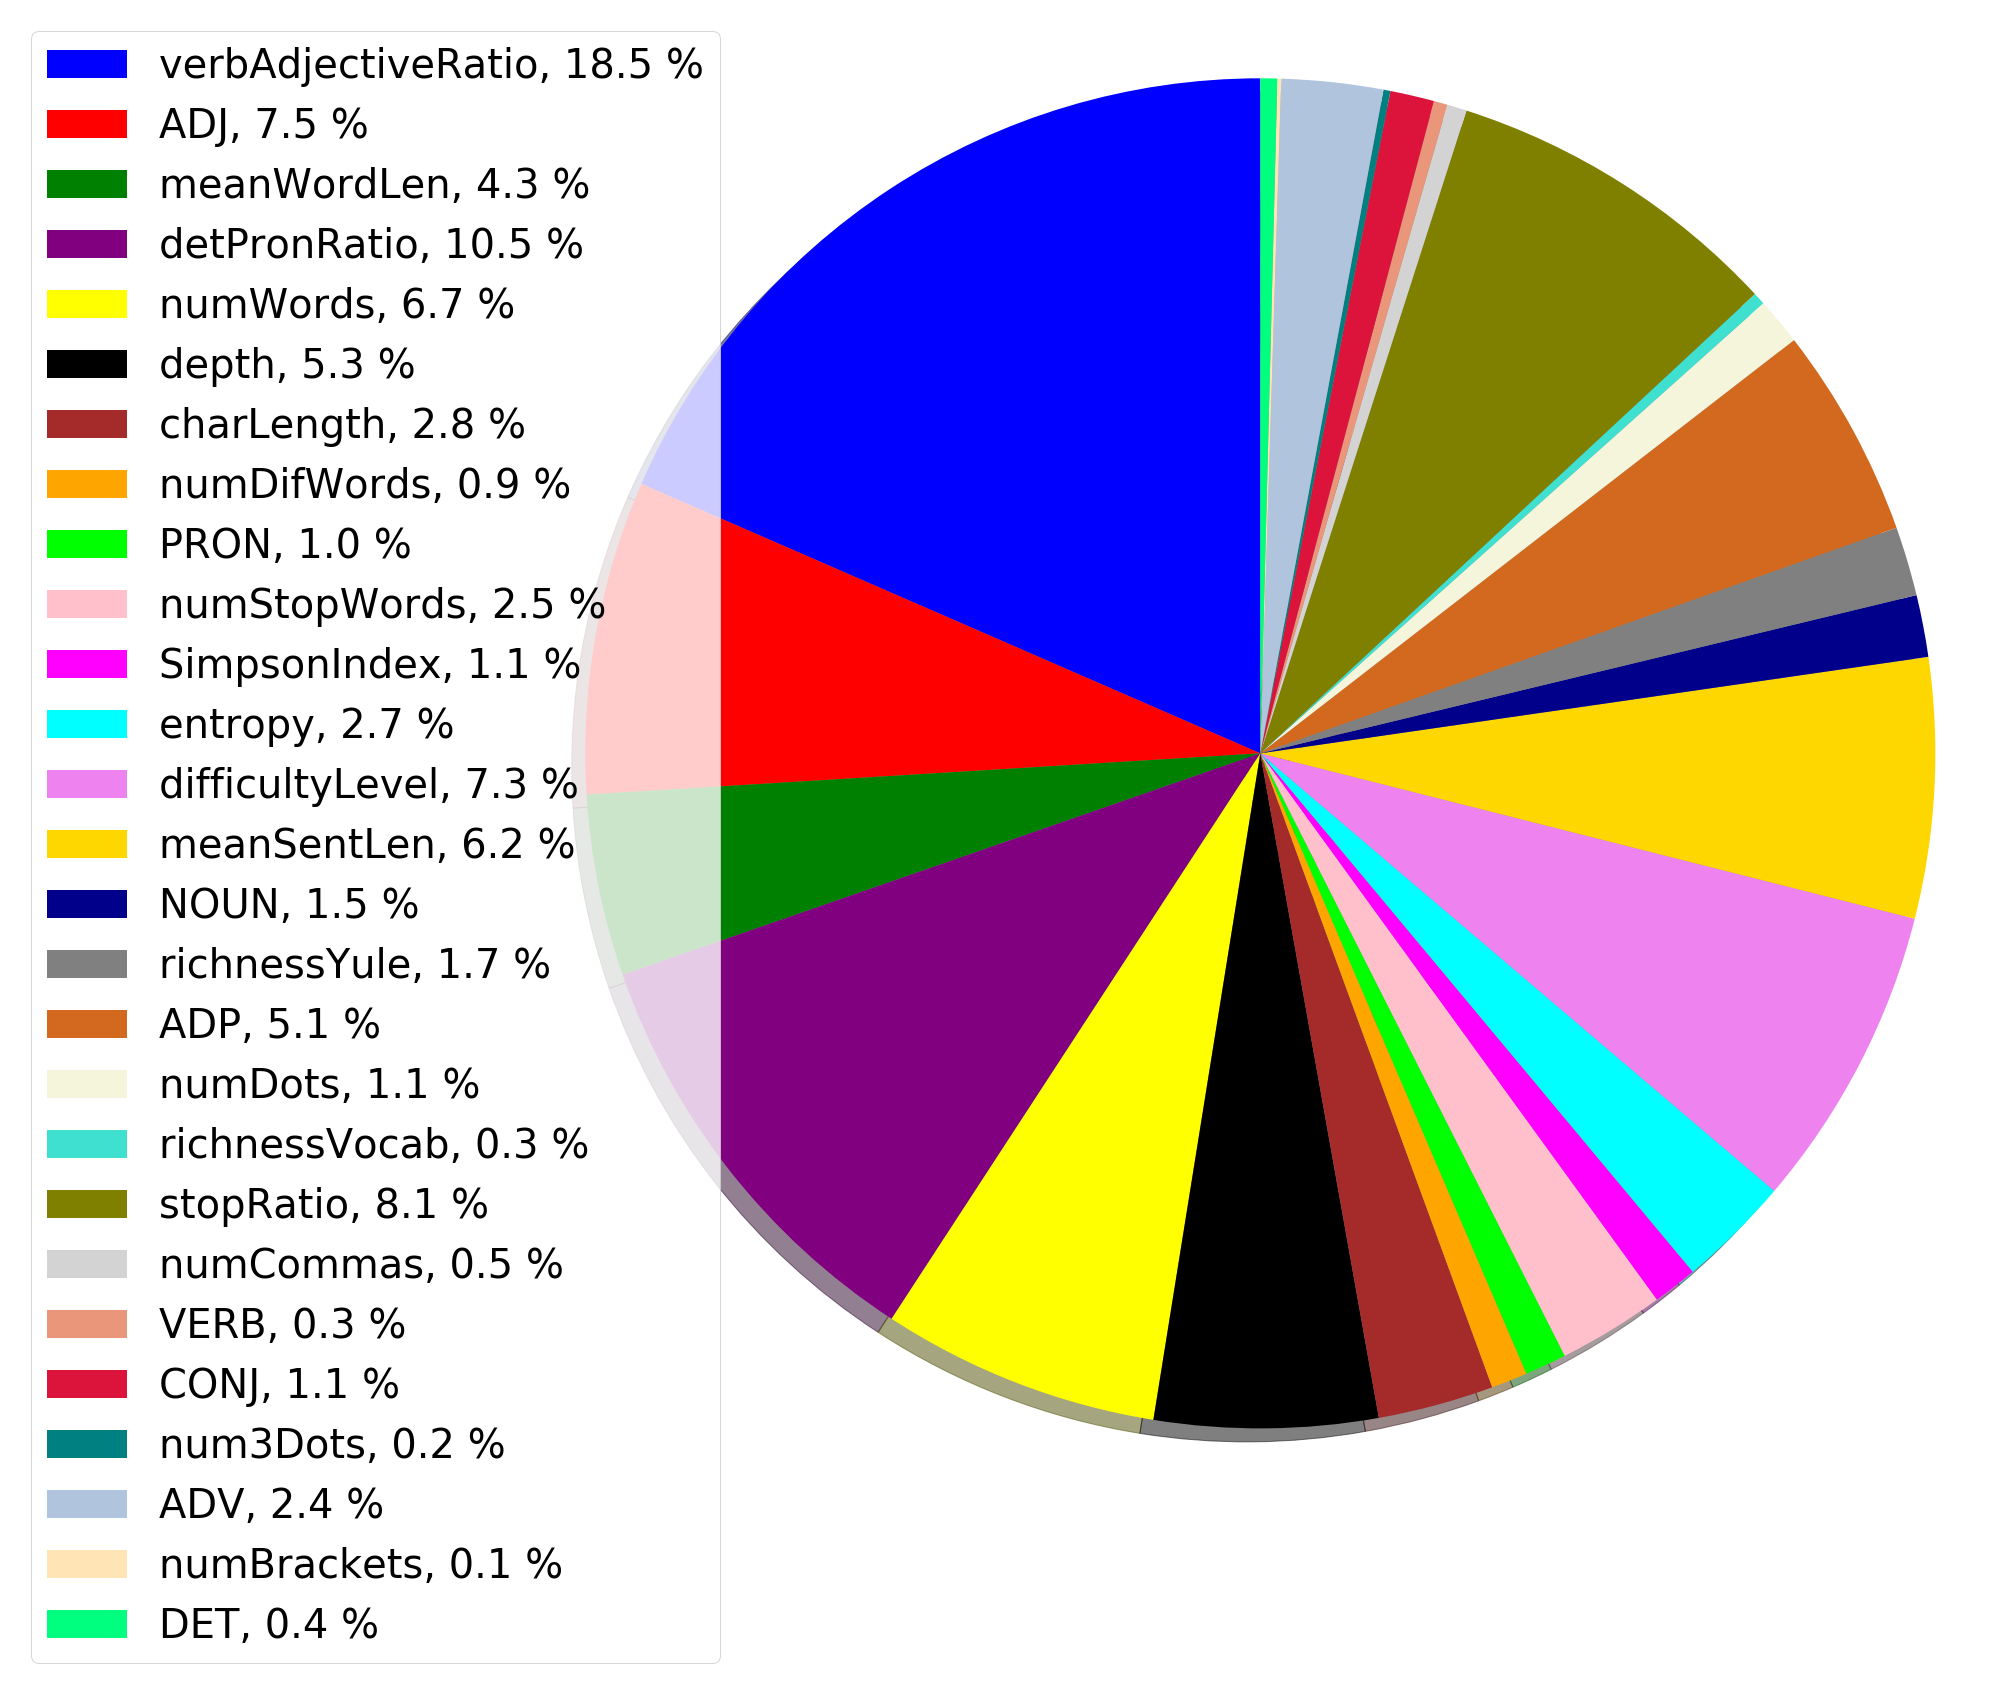
\includegraphics[width=0.8\textwidth]{Imagenes/Bitmap/DecisionTrees/pie28.png}}%
	\caption{Distribution of normalised feature importance with 28 features}%
	\label{fig:nfi28}
\end{figure}

As we can observe, the \textit{numSemiColon} characteristic has no importance in our constructed tree. Besides, \textit{verbAdjectiveRatio}, \textit{detPronRatio} and \textit{stopRatio} have the highest importance ratio and their related metrics (\textit{ADJ} and \textit{VERB}, \textit{DET} and \textit{PRON}, and \textit{numStopWords}, respectively) have a very small value. For this reason, we are able to claim that we can dispense with the related style features and \textit{numSemiColon} in order to describe the writing style. Therefore, we can construct another Decision Tree (by automatically taking a depth, as we have explained before) to calculate the importance ratio of each of the non-removed style markers. When we have the distribution of Gini Importance, we can removed again the non-important style metrics and those that have an extremely low importance ratio. By repeating this process, we are able to choose a small number of features which have a big importance ratio in the classification of the messages based on their recipients.

The learning curves of these iteration are all very similar to the one shown in Figure \ref{fig:learn28curve}. However, the evolution of the importance ratio of the style metrics is not uniform during all this iterative process. This behaviour could be seen in Figure \ref{fig:impcurv}.

\begin{figure}
	\centering%
	\centerline{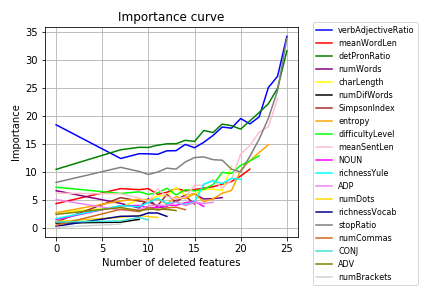
\includegraphics[width=0.9\textwidth]{Imagenes/Bitmap/DecisionTrees/limportancecurve.png}}%
	\caption{Evolution of importance ratio}%
	\label{fig:impcurv}
\end{figure}

Figure \ref{fig:impcurv} represents the importance ratio of each feature until it was removed from the set of style markers. The features that does not appear in the legend are those that were non-important in the first or second iteration, or were removed (such as the previously mentioned \textit{ADJ} and \textit{VERB}) before the second step.

Before detailing the different importance curves of each feature, there are some interesting general observations.
